\documentclass[12pt]{article}

\usepackage{lmodern}
\usepackage[utf8]{inputenc}
\usepackage[T1]{fontenc}
\usepackage[french]{babel}
\usepackage{url}
\usepackage{graphicx}
\usepackage{pifont}
\usepackage{subfig}

\graphicspath{ {./img/} }

\newcommand{\cmark}{\ding{51}}
\newcommand{\xmark}{\ding{55}}

\title{\textbf{Analyse de données d’eye-tracking en Réalité Virtuelle}}
\author{\Large{Adonis Stavridis}}
\date{Février 2021}

\begin{document}

% ------------------------------------------------------------------------------
% TITLEPAGE
% ------------------------------------------------------------------------------

\maketitle
\tableofcontents
\pagebreak

% ------------------------------------------------------------------------------
% INTRODUCTION
% ------------------------------------------------------------------------------

\section{Introduction}

L'eye-tracking \cite{wiki:eye_tracking}, ou oculométrie, est une technologie
qui permet de reconnaître la position du regard d'un individu dans un
environnement virtuel ou réel. Elle fournit un moyen de suivre les processus
attentionnels d'un utilisateur et permet d'établir une interface entre
Homme et machine. Cette technique peut être très utilisée pour les études liées
au système visuel humain, à la psychologie, au marketing et au design. Elle est
dèjà utilisée dans les jeux vidéos. Bien que cette technologie soit bien connue
et utilisée dans de multiples domaines de recherche, elle est encore peu
exploitée dans le domaine de la réalité virtuelle.

\bigskip
Déterminer la position du regard d'un individu dans un environnement permet
d'effectuer des études quantitatives et qualitatives sur de multiples supports,
et ainsi, de comprendre les cognitions et comportements humains dans différentes
situations. L'eye-tracking s'avère donc être très pratique pour étudier la
saillance des éléments présents dans les environnements virtuels. Cependant,
certaines études ont besoin d'un environnement plus réaliste. La réalité
virtuelle ajoute une nouvelle couche d'immersion, permettant à un individu de
se sentir et agir de façon plus réaliste. La réalité virtuelle permettrait
alors de livrer des résultats beaucoup plus fiables pour certains domaines, et
ainsi pousser à l'avancement des recherches sur le comportement humain.

\bigskip
L'objectif de ce travail consiste à développer des outils d'analyse des données
d'oculométrie afin de comparer le regard face à un écran ou dans un
environnement de réalité virtuelle. La visualisation et l'analyse des données
oculaires, peut être effectuée en temps réel ou par l'intermédiaire d'une
application. En vue de ce travail de recherche, un premier environnement (cf.
Figure \ref{fig:environnement}) a déjà été mis au point pour recueillir des
données d'eye-tracking sur un écran d'ordinateur, mais aussi dans un
environnement de réalité virtuelle. Un individu se place devant un écran et
observe différents supports, quant à la réalité virtuelle, l'individu porte un
casque et se retrouve dans ce même environnement face à un écran, cette fois-ci,
dans un monde virtuel. A partir des données recueillies au cours de sessions
exprimentales, il faudrait générer des supports (images et graphiques)
qui rassemblent toutes les informations nécessaires pour une analyse compléte de
l'étude. Il existe certaines bibliothèques et logiciels qui permettent de
traiter ces données, mais toutes ne présentent pas les mêmes fonctionnalités.

\begin{figure}[htpb]
  \centering
  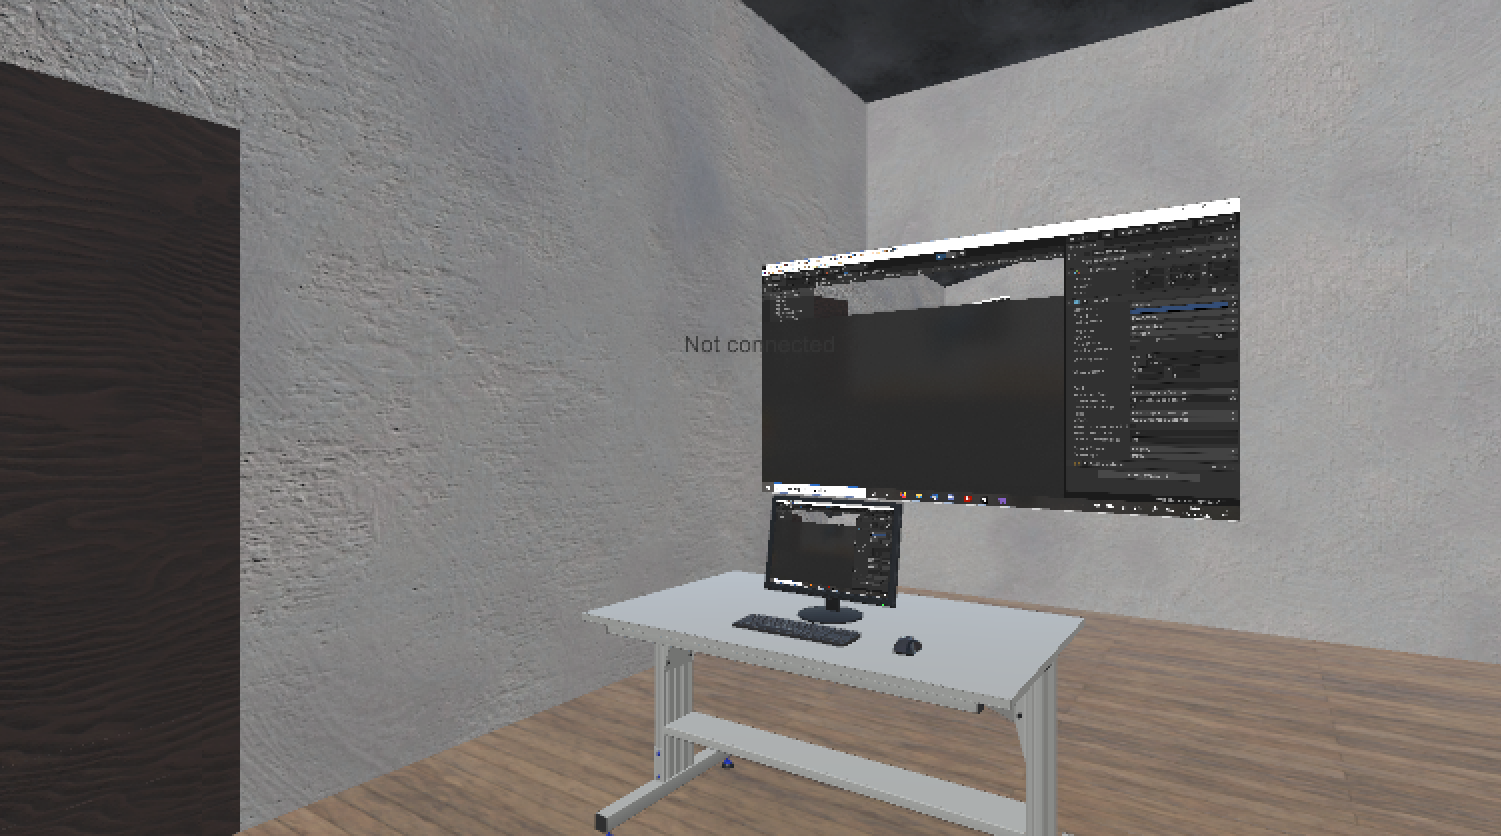
\includegraphics[width=0.75\textwidth,keepaspectratio=true]{environnement.png}
  \caption{Rendu de l'environnement mis en place en réalité virtuelle pour
    effectuer des mesures d'oculométrie \cite{img:environnement}.}
  \label{fig:environnement}
\end{figure}

\bigskip
Il convient dans un premier temps de sélectionner l'outil qui possède les
meilleurs atouts pour réaliser ces supports. Pour cela, il faut d'abord
comprendre comment sont récupérées les données, comment elle sont structurées
et puis identifier les types de support pertinents pour une analyse compléte,
afin de déterminer la bibliothèque la plus intéressante à utiliser pour
accomplir ce travail.

% ------------------------------------------------------------------------------
% CAPTEURS
% ------------------------------------------------------------------------------

\section{Capteurs}

L'eye-tracking est permis grâce à des émetteurs spéciaux qui envoient des rayons
infrarouges (non perceptibles par l'œil humain) vers les yeux d'un individu.
Ces rayons sont alors réfléchis par les yeux et les capteurs, à leur réception,
calculent la direction des yeux et peuvent ainsi déterminer la direction du
regard au fil du temps. Grâce à un logiciel intégré aux capteurs, le dispositif
va déterminer la position du regard dans un environnement d'étude, que ce soit
un écran ou un monde virtuel.

\bigskip
Les deux types de capteurs utilisés dans ce travail sont les suivants :
\begin{itemize}
  \item Des capteurs pour écrans : ce sont les capteurs les plus basiques. Ils
        sont placés au-dessus ou en-dessous d'un écran et orientés vers les yeux
        d'un individu. Ils permettent de suivre le regard sur un écran, donc
        dans un environnement à deux dimensions.
  \item Des capteurs intégrés à des casques de réalité virtuelle : ce sont des
        capteurs similaires aux précédents, mais qui ont été modifiés pour
        s'intégrer dans des casques de réalité virtuelle et observer les yeux à
        une distance beaucoup plus courte. Ces capteurs permettent de suivre le
        regard dans un environnement virtuel à trois dimensions. Un avantage à
        cette technologie est le rendu fovéal \cite{wiki:foveated_rendering}.
\end{itemize}

\bigskip
La plupart des produits liés à l'eye-tracking sont distribués par des
entreprises telles que Tobii \cite{tobii} et HTC Vice \cite{htc_vive_pro_eye}.
Ces solutions peuvent être utilisées dans plusieurs domaines \cite{yt:tobii_vr}
: les capteurs pour écrans peuvent être utiles pour étudier le regard d'un
individu sur une page web, par exemple, et ainsi déterminer les régions les
plus attrayantes ou non. Les casques de réalité virtuelle avec capteurs
intégrés sont quant à eux utilisés dans des situations d'entraînement ou des
circonstances difficilement réalisables dans le monde réel.

\begin{figure}[htpb]
  \centering
  \subfloat{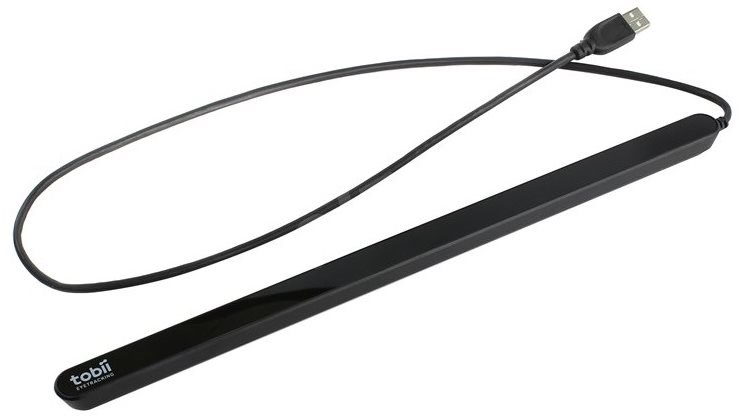
\includegraphics[width=5cm]{tobii.jpeg}}
  \qquad
  \subfloat{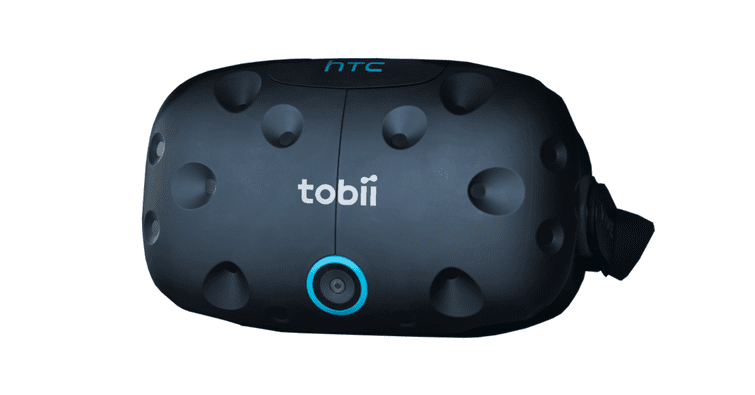
\includegraphics[width=5cm]{htcvive.png}}
  \caption{Capteur Tobii \cite{img:tobii} pour écrans (à gauche) et casque HTC
    Vive \cite{img:htcvive} pour la réalité virtuelle (à droite).}
  \label{fig:materiel}
\end{figure}

Il existe plusieurs types de capteurs, certains plus spécialisés dans certains
domaines que d'autres. Les capteurs sont fournis avec des logiciels capables de
produire toutes les données nécessaires pour les analyser. Dans le cadre de ce
travail, les capteurs utilisés sont une barre de tracking Tobii pour écrans et
un casque HTC Vive avec capteur intergré pour la réalité virtuelle (cf. Figure
\ref{fig:materiel}).

% ------------------------------------------------------------------------------
% ANALYSE DES DONNÉES
% ------------------------------------------------------------------------------

\section{Analyse des données}

Après avoir récupéré les données brutes d'une séance d'oculométrie, il faut
pouvoir les analyser afin d'en tirer des informations pertinentes. Les
données sont une série de valeurs numériques (cf. Figure \ref{fiées de façon plus explicite.}),
représentants les positions du regard dans un environnement, mais sont
difficilement compréhensibles telles quelles. Pour cela, il serait beaucoup
plus intéressant de transformer les données en des réprésentations imagées et
graphiques de différents types. Il existe différentes mesures et termes
utilisés pour analyser le regard \cite{imotions:metrics}, chacune organisant
les données de façon à avoir une analyse compléte, étudiant tous les aspects du
regard.

\begin{figure}[htpb]
  \begin{verbatim}
    <temps> : <positionX>, <positionY>
    0.00 : 50, 50
    0.25 : 43, 64
    0.50 : 38, 75
    0.75 : 41, 66
    1.00 : 38, 59
    1.25 : 35, 51
    1.50 : 29, 44
    1.75 : 24, 40
    2.00 : 20, 33
  \end{verbatim}
  \caption{Exemple de données fournies par les logiciels de capteurs, avec une
    indication du temps et de la position du regard (en pixels ou en
    pourcentages) sur l'axe horizontal et vertical.}
  \label{fiées de façon plus explicite.}
\end{figure}

\subsection{Points de fixation}

L'un des indicateurs les plus utilisés pour représenter le regard au fil du
temps sont les points de fixation. Ce sont des mesures qui consistent à indiquer
le point de focalisation d'un individu à un instant donné. Un capteur qui
collectionne des données avec un taux d'échantillonage de 120hz, par exemple, va
fournir en sortie 120 points de fixations par seconde. Il faut donc faire une
organisantion de ces points en fonctions du temps et de l'espace. La quantité de
points de fixations montre à quel point l'attention visuelle a été portée en une
région.

\subsection{Séquence de fixations}

Étudier la séquence de ces points de fixations serait également intéressant. Un
individu va d'abord fixer son regard sur les régions les plus prioritaires et va
se construire l'environnement petit à petit, en se concentrant sur plusieurs
zones. L'ordre d'attention est important dans la recherche car elle reflète de
l'intérêt d'un individu sur une région et met en avant les objets les plus
captivants au premier regard. Le premier point de fixation peut être aléatoire,
mais les zones de fixations qui suivent peuvent parfois être prédites (pour
une interface utilisateur, par exemple).

\subsection{Heatmaps}

Une autre représentation très importante est la distribution des points de
fixation, sous la forme d'une heatmap. Un gradient de couleur est placé sur
l'environnement original indiquant du rouge au bleu les régions les plus
attrayantes (cf. Figure \ref{fig:heatmap}). Ces heatmaps sont un moyen très
simple de différencier les régions qui attirent le plus l'attention. C'est
l'une des représentations les plus importantes pour comprendre la saillance des
éléments dans un environnement.

\begin{figure}[ht]
  \centering
  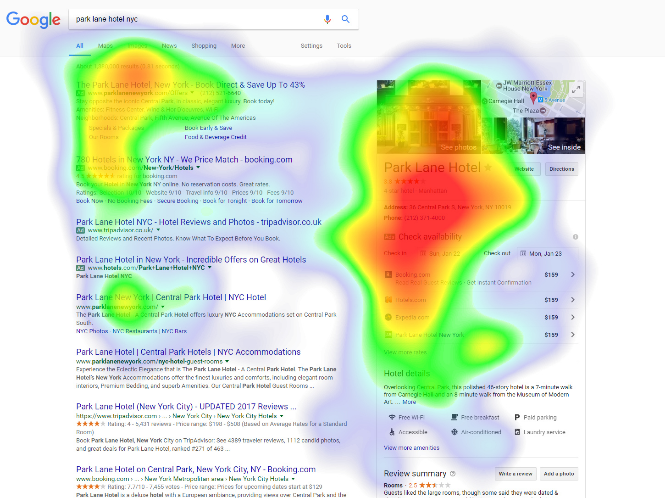
\includegraphics[width=0.75\textwidth,keepaspectratio=true]{heatmap.png}
  \caption{Exemple de heatmap sur une page de recherche sur Google
    \cite{img:heatmap}.}
  \label{fig:heatmap}
\end{figure}

\subsection{Zones d'intérêt}

Une zone d'intérêt n'est pas vraiment une représentation mais un outil qui
permet de spécifier des zones, des objets au préalable, pour en extraire leurs
mesures. C'est un outil pratique pour bien séparer les différentes zones d'un
environnement d'étude, et déterminer les régions les plus importantes. Dans les
mesures de chaque zone, il serait intéressant d'y calculer :

\begin{itemize}
  \item le délai à la première fixation : le temps qu'un individu à mis
        depuis le début pour fixer une zone pour la première fois.
  \item la durée de fixation : la somme du temps qu'un individu a passé a
        fixer une zone.
  \item le nombre de fixations : le nombre de fois qu'un individu à fixé
        une zone, puisque le regard peut fixer une zone, la quitter et
        puis revenir dessus.
\end{itemize}

\bigskip
Il existe donc plusieurs façons d'organiser les données et de les représenter
pour faciliter leur compréhension et permettre d'en tirer les bonnes
conclusions, en prenant en compte tous les aspects de l'étude du regard. Il
serait également intéressant de créer plusieurs graphiques pour représenter ces
données de façon plus explicite.

% ------------------------------------------------------------------------------
% LOGICIELS
% ------------------------------------------------------------------------------

\section{Logiciels}

Pour pouvoir analyser les données et créer ces réprésentations il faudrait soit
utiliser des bibliothèques ou des applications déjà disponibles
\cite{imotions:software}, soit créer les outils. Heureusement, il existe
certains logiciels open-source, ou gratuits uniquement, permettant d'effectuer
un minimum d'analyse de données. L'objectif est donc de déterminer quel
logiciel est le plus intéressant à utiliser dans le cadre de ce travail,
pour étudier le regard sur un écran, mais aussi dans un environnement de
réalité virtuelle.

\subsection{GazePointer}

Gazepointer \cite{gazepointer} est une application libre qui permet d'effectuer
de l'eye-tracking principalement. Il existe une fonctionnalité intégrée au
logiciel qui permet d'effectuer des séances de suivi du regard, et génerer une
heatmap des fixations. Cependant c'est la seule analyse possible. De plus,
c'est un logiciel qui fonctionne indépendamment, et non pas une bibliothèque :
ses outils ne sont pas accessibles en dehors de l'application. De plus, le
logiciel fonctionne uniquement avec des webcams. Gazepointer permet d'analyser
des données d'oculométrie, mais son implémentation n'est pas optimale dans le
cadre de ce travail, avec les capteurs disponibles, et ne permet pas du tout
l'oculométrie en réalité virtuelle.

\subsection{Ogama}

Ogama \cite{ogama} est une application open-source qui permet d'enregistrer et
d'analyser des données d'oculométrie et de mouvements de souris. Le logiciel
permet essentielment de créer des cartes de fixations et des zones d'intérêt,
et du calcul de saillance, pour déterminer quelles régions sont les plus
attrayantes. Il accepte toutes de données enregistrées en format ASCII, et, en
plus, le logiciel est certifié de fonctionner avec plusieurs logiciels
d'oculométrie et capteurs sur le marché tels que Tobii. Ogama est donc
certainement intéressant pour pouvoir importer et analyser des données
facilement. Cependant, ce n'est pas une bibliothèque et ne permet donc pas
autant de flexibilité.

\subsection{PyGaze}

PyGaze \cite{pygaze} est quant à elle une boîte à outil Python, permettant
également d'effectuer du suivi de regard et analyser les données. La
fonctionnalité la plus intéressante de cette bibliothèque est l'outil
d'analyse des données. PyGaze permet d'afficher les données sous forme de
cartes de fixations, des cartes de séquence de fixations, des heatmaps,
mais aussi sous forme brute pour rendre visible tout l'espace que la
trajectoire oculaire a traversé. Le code de PyGaze est open-source et il est
donc possible de se baser sur cette bibliothèque pour développer d'autres
outils. De plus, elle supporte des SDK tels que celui de Tobii. Les façons de
représenter les données sont multiples, et il serait donc possible de
l'utiliser pour créer des outils d'analyse en réalité virtuelle.

\subsection{GazeParser}

GazeParser \cite{gazeparser} est une bibliothèque d'analyse des données du
regard qui permet essentielment de récupérer les données et les visualiser sous
forme de graphiques. Ceci peut être pratique pour avoir une approche plus brute
des données. GazeParser permet aussi d'appliquer des filtres sur les données
pour réduire le bruit et effectuer une analyse plus correcte. Elle peut être
utilisée avec le langage Python, pour effectuer, au l'inverse des
réprésentations imagées, des graphiques qui affichent les données exactes.


\bigskip
\begin{table}[htpb]
  \begin{center}
    \begin{tabular}{|c||c|c|c|}
      \hline
      \multicolumn{4}{|c|}{Comparaison des logiciels}             \\
      \hline
      Logiciels   & Flexibilité   & Analyse       & Documentation \\
      \hline
      GazePointer & \xmark        & \cmark        & \cmark        \\
      Ogama       & \xmark        & \cmark \cmark & \cmark        \\
      PyGaze      & \cmark \cmark & \cmark \cmark & \cmark \cmark \\
      GazeParser  & \cmark        & \cmark \cmark & \cmark        \\
      \hline
    \end{tabular}
    \caption{Comparaison des logiciels en fonction de leur flexibilité
      (possibilité d'être manipulé librement), leur capacité de géneration de
      d'analyse des données et leur documentation.}
    \label{tab:comparaison}
  \end{center}
\end{table}

Il existe donc plusieurs applications et bibliothèques gratuites permettant
d'effectuer une analyse sur les jeux de données créés par les capteurs. Il
existe également des logiciels payants, mais ceux-ci sont hors de portée dans le
cadre de ce travail. Après comparaison entre les logiciels (cf. Table
\ref{tab:comparaison}), une bibliothèque en particulier se démarque. PyGaze est
le candidat idéal ici, puisque elle permettrait d'être utilisée pour analyser
les données librement et facilement, afin de créer des réprésentations visuelles
du regard. Sinon, GazeParser pour servir pour effectuer des graphiques et
représenter les données de façon plus chiffrée.

% ----------------------------------------------------------------------------
% CONCLUSION
% ----------------------------------------------------------------------------

\section{Conclusion}

L'eye-tracking est une technologie qui présente un fort potentiel en recherche,
mais les études dans le domaine de la réalité virtuelle restent peu nombreuses.
L'objectif de ce travail étant de développer des outils d'analyse de données
d'oculométrie, il faut choisir des bibliothèques capables de créer des représentations des données récupérées, pour des étude d'eye-tracking sur écran et en réalité virtuelle également. La bibliothèque la plus intéressante à utiliser est PyGaze : elle permet de génerer plusieurs cartes d'analyse et pourrait être une très utile pour développer des outils d'analyse en réalité virtuelle. GazeParser pourrait être tout à fait utile pour génerer des graphiques. Grâce aux capteurs Tobii et HTC Vive, il sera possible d'enregistrer des données, qui seront analysés par la suite pour enfin créer des représentations claires et précises, afin de comparer les différences du regard humain sur un écran et dans un monde virtuel.

% ----------------------------------------------------------------------------
% BIBLIOGRAPHIE
% ----------------------------------------------------------------------------

\bibliographystyle{unsrt}
\bibliography{recherches}

\end{document}
